\section{Piecewise Aggregate Approximation}
The algorithms for time series discretization explained in this chapter all depend on the \ac{PAA} as a preprocessing step. The \ac{PAA} first standardizes the original time series before it transforms it to an intermediate representation \cite{PAA_Keogh}. This intermediate representation is then used by the time series discretization algorithms to obtain the discretized representation of the original time series. \newline
\subsection*{Main Procedure}
Let $X = x_1, ..., x_N$ be a standardized time series of length $N \geq 1$. Further, consider X as a point in an $N$-dimensional space. Then, the main idea of the \ac{PAA} is to project X onto a lower-dimensional space of dimensionality $1 \leq n \leq N$ \cite{PAA_Keogh}. \newline
First, a non-overlapping sliding window of length $1 \leq w \leq N$ is used to partition $X$ into subsequences of equal length \cite{PAA_Keogh}. Assuming that $N$ is divisible by $w$, this results in $n = N \cdot w^{-1}$ subsequences of length $w$. The final step is to compute the mean of the $w$ points of each subsequence to get an approximation of the subsequence (see Figure \ref{fig:PAA}) \cite{PAA_Yi_Faloutsos}. \newline
Let $\overline{x}_i$ $(1 \leq i \leq n)$ be the mean of the $w$ points of the $i$-th extracted subsequence from $X$. Then, $\overline{X} = \overline{x}_1, ..., \overline{x}_n$ is the resulting time series in the lower-dimensional space of dimensionality $n$, where $\overline{x}_i$ is computed by \cite{PAA_Keogh}:
\begin{equation}
\overline{x}_i = \frac{n}{N} \sum_{j=\frac{N}{n}(i-1)+1}^{\frac{N}{n}i}\mkern-24mu x_j
\end{equation}
\begin{figure}[htb]
\centering
\includegraphics[width=0.8\textwidth]{discretization/paa/paa_sliding_window_short.pdf}
\caption[Piecewise Aggregate Approximation - Sliding Window]{The original time series is partitioned by a non-overlapping sliding window into subsequences of equal length. For each subsequence the mean of its points is computed. These means (green squares) are the points of the time series that is the result of the \ac{PAA} \cite{PAA_Keogh}.} 
\label{fig:PAA}
\end{figure}
\subsection*{Strategies for Time Series of Indivisable Length}
The assumption that $N$ is divisible by $w$ is not a requirement of the \ac{PAA}, but it simplifies notation and understanding \cite{PAA_Keogh}. \newline
One strategy when $N$ is not divisible by $w$ is to append additional points with a value of zero to $X$ until $N$ is divisible by $w$ \cite{PAA_Yi_Faloutsos}. This is a straightforward strategy. But, on the other hand, the mean computed for the last extracted subsequence will be distorted. The extent of this distortion will be greater the closer the number of additionally appended points is to $w$. \newline
Another strategy is to truncate the points of $X$ until $N$ is divisible by $w$. This is also a straightforward strategy, but the time series is modified and information, in the form of time series points, is lost. \newline
The strategy that is used for the evaluation in this thesis (see Chapter \ref{evaluation_chapter}) tries to find a compromise between the strategies mentioned above. First, the window length $w$ is applied on the time series. Then, depending on the number of points contained in the last extracted subsequence, it is decided to truncate these points or to compute the mean of these points. When this number of points is greater than $\frac{w}{2}$, the mean of these points is computed, otherwise these points along with the last extracted subsequence are truncated. Due to this threshold of $\frac{w}{2}$, this strategy is straightforward, does not distort the mean computed for the last extracted subsequence, and limits the loss of information.
\subsection*{Role of the Window Length as Input Parameter} \label{parameter_window_length}
Since the \ac{PAA} is a downsampling approach, $\overline{X}$ is an approximation of $X$ which incurs a loss of information \cite{PAA_Yi_Faloutsos}. On the other hand, this approximation also incurs a gain in free memory. From $n \leq N$ it follows that storing $\overline{X}$ needs at most as much memory as storing $X$. These two observations imply a trade-off between the loss of information and the gain in free memory incurred when applying the \ac{PAA} on $X$ \cite{SAX_Lin}. \newline
The decisive parameter that affects this trade-off is the window length $w$ \cite{SAX_Lin}. Qualitatively, as $w$ increases more information is lost, but less memory for storing $\overline{X}$ is required, because less means $\overline{x}_i$ are computed to approximate $X$. On the other hand, as $w$ decreases less information is lost, but more memory for storing $\overline{X}$ is required, because more means $\overline{x}_i$ are computed to approximate $X$. When assigning each point of an extracted subsequence the corresponding mean of the subsequence, this trade-off can be visualized (see Figure \ref{fig:PAA_inverse}) \cite{SAX_Lin}. \newline
Note that $\overline{X}$ is the mean of $X$ for the extreme case of $w = N$ and $\overline{X} = X$ for the extreme case of $w = 1$, meaning that each point of $X$ is its own mean \cite{PAA_Keogh}.
\begin{figure}[htb]
\centering
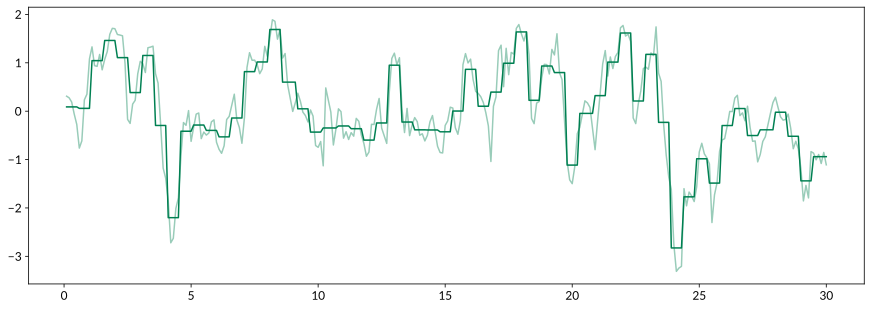
\includegraphics[width=0.8\textwidth]{discretization/paa/paa_inverse_transformation.pdf}
\caption[Piecewise Aggregate Approximation - Effect of Window Size]{The original time series in these two plots consists of 300 points. In the plot above a window length of $w = 5$ (i.e. five points) is used to extract the subsequences, while in the plot below a window length of $w = 10$ (i.e. ten points) is used. The approximation in the plot above captures more fine-grained characteristics of the original time series like local extrema, while the approximation in the plot below is more coarse-grained. However, the approximation in the plot above is created with 60 points (i.e means) compared to 30 points (i.e. means) that are used for the approximation in the plot below.} 
\label{fig:PAA_inverse}
\end{figure}
\subsection*{Time Complexity}
For the \ac{PAA}, $\frac{N}{w}$ subsequences need to be extracted from $X$ while each subsequence contains $w$ points. Further, the computation of the mean is linear in the number of points. Hence, the \ac{PAA} has a time complexity of $\mathcal{O}(\frac{N}{w}\cdot w) = \mathcal{O}(N)$ \cite{PAA_Keogh}.
